%% BioMed_Central_Tex_Template_v1.06
%%                                      %
%  bmc_article.tex            ver: 1.06 %
%                                       %

%%IMPORTANT: do not delete the first line of this template
%%It must be present to enable the BMC Submission system to
%%recognise this template!!

%%%%%%%%%%%%%%%%%%%%%%%%%%%%%%%%%%%%%%%%%
%%                                     %%
%%  LaTeX template for BioMed Central  %%
%%     journal article submissions     %%
%%                                     %%
%%          <8 June 2012>              %%
%%                                     %%
%%                                     %%
%%%%%%%%%%%%%%%%%%%%%%%%%%%%%%%%%%%%%%%%%


%%%%%%%%%%%%%%%%%%%%%%%%%%%%%%%%%%%%%%%%%%%%%%%%%%%%%%%%%%%%%%%%%%%%%
%%                                                                 %%
%% For instructions on how to fill out this Tex template           %%
%% document please refer to Readme.html and the instructions for   %%
%% authors page on the biomed central website                      %%
%% http://www.biomedcentral.com/info/authors/                      %%
%%                                                                 %%
%% Please do not use \input{...} to include other tex files.       %%
%% Submit your LaTeX manuscript as one .tex document.              %%
%%                                                                 %%
%% All additional figures and files should be attached             %%
%% separately and not embedded in the \TeX\ document itself.       %%
%%                                                                 %%
%% BioMed Central currently use the MikTex distribution of         %%
%% TeX for Windows) of TeX and LaTeX.  This is available from      %%
%% http://www.miktex.org                                           %%
%%                                                                 %%
%%%%%%%%%%%%%%%%%%%%%%%%%%%%%%%%%%%%%%%%%%%%%%%%%%%%%%%%%%%%%%%%%%%%%

%%% additional documentclass options:
%  [doublespacing]
%  [linenumbers]   - put the line numbers on margins

%%% loading packages, author definitions

%\documentclass[twocolumn]{bmcart}% uncomment this for twocolumn layout and comment line below
\documentclass{bmcart}

%%% Load packages
%\usepackage{amsthm,amsmath}
%\RequirePackage{natbib}
%\RequirePackage[authoryear]{natbib}% uncomment this for author-year bibliography
%\RequirePackage{hyperref}
\usepackage[utf8]{inputenc} %unicode support
%\usepackage[applemac]{inputenc} %applemac support if unicode package fails
%\usepackage[latin1]{inputenc} %UNIX support if unicode package fails
\usepackage{graphicx}

%% These have been added at the request of the MIT Libraries, because
%% some PDF conversions mess up the ligatures.  -LB, 1/22/2014
\usepackage{cmap}
\usepackage[T1]{fontenc}
\pagestyle{plain}

\usepackage{graphicx}
\usepackage[utf8]{inputenc}
\usepackage[T1]{fontenc} 
%\usepackage[latin1]{inputenc}
\usepackage{pifont} 
\usepackage{import}
\usepackage{amsmath}
\usepackage{multirow}
\usepackage{graphicx,url}
\usepackage{placeins}
\usepackage{adjustbox}
\usepackage[english]{babel}
\usepackage{lipsum}
\usepackage{multicol}
\usepackage{textcomp}
\usepackage{listings}
\usepackage{caption}
\usepackage{amsmath}
\usepackage{calc} 
\usepackage{array,url,kantlipsum}
\usepackage{algorithm}
\usepackage{algpseudocode}
\usepackage{lscape}
\usepackage{array}
\usepackage{natbib}
\usepackage{longtable}
\usepackage{booktabs}
\usepackage{txfonts}
\usepackage{colortbl}%
  \newcommand{\myrowcolour}{\rowcolor[gray]{0.925}}
\newenvironment{Figure}
  {\par\medskip\noindent\minipage{\linewidth}}
  {\endminipage\par\medskip}
  
\lstset{
language=Java,
basicstyle=\small\ttfamily,
numbers=left,
numbersep=5pt,
xleftmargin=20pt,
frame=tb,
framexleftmargin=20pt
}

\renewcommand*\thelstnumber{\arabic{lstnumber}:}

\DeclareCaptionFormat{mylst}{\hrule#1#2#3}
\captionsetup[lstlisting]{format=mylst,labelfont=bf,singlelinecheck=off,labelsep=space,font={normalsize,tt}}

\usepackage[framemethod=tikz]{mdframed}
\usepackage{lipsum}

\extrafloats{100}

%%%%%%%%%%%%%%%%%%%%%%%%%%%%%%%%%%%%%%%%%%%%%%%%%
%%                                             %%
%%  If you wish to display your graphics for   %%
%%  your own use using includegraphic or       %%
%%  includegraphics, then comment out the      %%
%%  following two lines of code.               %%
%%  NB: These line *must* be included when     %%
%%  submitting to BMC.                         %%
%%  All figure files must be submitted as      %%
%%  separate graphics through the BMC          %%
%%  submission process, not included in the    %%
%%  submitted article.                         %%
%%                                             %%
%%%%%%%%%%%%%%%%%%%%%%%%%%%%%%%%%%%%%%%%%%%%%%%%%


\def\includegraphic{}
\def\includegraphics{}



%%% Put your definitions there:
\startlocaldefs
\endlocaldefs


%%% Begin ...
\begin{document}

%%% Start of article front matter
\begin{frontmatter}

\begin{fmbox}
\dochead{Research}

%%%%%%%%%%%%%%%%%%%%%%%%%%%%%%%%%%%%%%%%%%%%%%
%%                                          %%
%% Enter the title of your article here     %%
%%                                          %%
%%%%%%%%%%%%%%%%%%%%%%%%%%%%%%%%%%%%%%%%%%%%%%

\title{Improving Search-Based Stress Testing using Q-Learning and Hybrid Metaheuristic Approach}

%%%%%%%%%%%%%%%%%%%%%%%%%%%%%%%%%%%%%%%%%%%%%%
%%                                          %%
%% Enter the authors here                   %%
%%                                          %%
%% Specify information, if available,       %%
%% in the form:                             %%
%%   <key>={<id1>,<id2>}                    %%
%%   <key>=                                 %%
%% Comment or delete the keys which are     %%
%% not used. Repeat \author command as much %%
%% as required.                             %%
%%                                          %%
%%%%%%%%%%%%%%%%%%%%%%%%%%%%%%%%%%%%%%%%%%%%%%

\author[
   addressref={aff1},                   % id's of addresses, e.g. {aff1,aff2}
   corref={aff1},                       % id of corresponding address, if any
   noteref={n1},                        % id's of article notes, if any
   email={naubergois@gmail.com}   % email address
]{\inits{NG}\fnm{Nauber} \snm{Gois}}
\author[
   addressref={aff1},
   email={porfirio@unifor.br}
]{\inits{PP}\fnm{Pedro} \snm{Porfírio}}
\author[
   addressref={aff1},
   email={acoelho@unifor.br}
]{\inits{AC}\fnm{André} \snm{Coelho}}


%%%%%%%%%%%%%%%%%%%%%%%%%%%%%%%%%%%%%%%%%%%%%%
%%                                          %%
%% Enter the authors' addresses here        %%
%%                                          %%
%% Repeat \address commands as much as      %%
%% required.                                %%
%%                                          %%
%%%%%%%%%%%%%%%%%%%%%%%%%%%%%%%%%%%%%%%%%%%%%%

\address[id=aff1]{%                           % unique id
  \orgname{Departamento de Informática Aplicada, UNIFOR}, % university, etc
  \street{Av. Washington Soares, 1321},                     %
  %\postcode{}                                % post or zip code
  \city{Fortaleza},                              % city
  \cny{BR}                                    % country
}

%%%%%%%%%%%%%%%%%%%%%%%%%%%%%%%%%%%%%%%%%%%%%%
%%                                          %%
%% Enter short notes here                   %%
%%                                          %%
%% Short notes will be after addresses      %%
%% on first page.                           %%
%%                                          %%
%%%%%%%%%%%%%%%%%%%%%%%%%%%%%%%%%%%%%%%%%%%%%%

\begin{artnotes}
%\note{Sample of title note}     % note to the article
\note[id=n1]{Equal contributor} % note, connected to author
\end{artnotes}

\end{fmbox}% comment this for two column layout

%%%%%%%%%%%%%%%%%%%%%%%%%%%%%%%%%%%%%%%%%%%%%%
%%                                          %%
%% The Abstract begins here                 %%
%%                                          %%
%% Please refer to the Instructions for     %%
%% authors on http://www.biomedcentral.com  %%
%% and include the section headings         %%
%% accordingly for your article type.       %%
%%                                          %%
%%%%%%%%%%%%%%%%%%%%%%%%%%%%%%%%%%%%%%%%%%%%%%

\begin{abstractbox}

\begin{abstract} 
Some software systems must respond to thousands or millions of concurrent requests. These systems must be properly tested to ensure that they can function correctly under the expected load. Performance degradation and consequent system failures usually arise in stressed conditions. Stress testing subjects the program to heavy loads. In this context, search-based testing is seen as a promising approach to verify timing constraints. In this paper, We propose a hybrid metaheuristic approach that uses genetic algorithms, simulated annealing, and tabu search algorithms in a collaborative model using Q-Learning to improve stress search-based  testing and  automation. The main goal of the research is to find scenarios that maximize the number of users in the application with a response time below the response time service level. A tool named IAdapter, a JMeter plugin used for performing search-based stress tests, was developed. Two experiments were conducted to validate the proposed approach.
\end{abstract}

%%%%%%%%%%%%%%%%%%%%%%%%%%%%%%%%%%%%%%%%%%%%%%
%%                                          %%
%% The keywords begin here                  %%
%%                                          %%
%% Put each keyword in separate \kwd{}.     %%
%%                                          %%
%%%%%%%%%%%%%%%%%%%%%%%%%%%%%%%%%%%%%%%%%%%%%%

\begin{keyword}
\kwd{Search-Based Test}
\kwd{Stress Testing}
\kwd{Hybrid metaheuristic}
\kwd{Q-Learning}
\end{keyword}

% MSC classifications codes, if any
%\begin{keyword}[class=AMS]
%\kwd[Primary ]{}
%\kwd{}
%\kwd[; secondary ]{}
%\end{keyword}

\end{abstractbox}
%
%\end{fmbox}% uncomment this for twcolumn layout

\end{frontmatter}

%%%%%%%%%%%%%%%%%%%%%%%%%%%%%%%%%%%%%%%%%%%%%%
%%                                          %%
%% The Main Body begins here                %%
%%                                          %%
%% Please refer to the instructions for     %%
%% authors on:                              %%
%% http://www.biomedcentral.com/info/authors%%
%% and include the section headings         %%
%% accordingly for your article type.       %%
%%                                          %%
%% See the Results and Discussion section   %%
%% for details on how to create sub-sections%%
%%                                          %%
%% use \cite{...} to cite references        %%
%%  \cite{koon} and                         %%
%%  \cite{oreg,khar,zvai,xjon,schn,pond}    %%
%%  \nocite{smith,marg,hunn,advi,koha,mouse}%%
%%                                          %%
%%%%%%%%%%%%%%%%%%%%%%%%%%%%%%%%%%%%%%%%%%%%%%

%%%%%%%%%%%%%%%%%%%%%%%%% start of article main body
% <put your article body there>

%%%%%%%%%%%%%%%%
%% Background %%
%%

\section{Introduction}

Many systems must support concurrent access to hundreds or thousands of users. Failure to provide scalable access to users may result in catastrophic failures and unfavorable media coverage \citep{Jiang2010}. 

The explosive growth of the Internet has contributed to the increased need for applications that perform at an appropriate speed. Performance problems are often detected late in the application life cycle, and the later they are discovered, the greater the cost is to fix them \citep{Molyneaux2009}.

The use of stress testing is an increasingly common practice owing to the fact that the increasing number of users. In this scenario, the inadequate treatment of a workload generated by concurrent or simultaneous access due to several users can result in highly critical failures and negatively affect the customer's perception of the company \citep{Draheim2006b} \citep{Jiang2010}. 

Stress testing determines the responsiveness, throughput, reliability, or scalability of a system under a given workload. The quality of the results of applying a given load testing to a system is closely linked to the implementation of the workload strategy. The performance of many applications depends on the load applied under different conditions. In some cases, performance degradation and failures arise only in stress conditions \citep{Garousi2010} \citep{Jiang2010}.


A stress test uses a set of workloads that consist of many types of usage scenarios and a combination of different numbers of users. A load is typically based on an operational profile. Different parts of an application should be tested under various parameters and stress conditions \citep{Babbar2011}. The correct application of a stress test should cover most parts of an application above the expected load conditions\citep{Draheim2006b}.

The stress testing process in the industry still follows a non-automated and ad-hoc model where the designer or tester is responsible for running the tests, analyzing the results and deciding which new tests should be performed \citep{Lewis2005}. 

Typically, performance testing is accomplished using test scripts, which are programs that test designers write to automate testing. These test scripts perform actions or mimic user actions on GUI objects of the system to feed input data. Current approaches to stress testing suffer from limitations. Their cost-effectiveness is highly dependent on the particular test scenarios that are used, and yet there is no support for choosing those scenarios. A poor choice of scenarios could lead to underestimating system response time thereby missing an opportunity to detect a performance problem \citep{Grechanik2012}.

Search-based testing is seen as a promising approach to verify timing constraints \citep{Afzal2009a}. A common objective of a stress search-based test is to find  scenarios that produce execution times that violate the specified timing constraints \citep{Sullivan}. 


This research proposes to extends the Hybrid Algorithm presented by Gois et al. \citep{Gois2016}. The research approach uses Q-Learning reinforcement learning technique (HybridQ algorithm) to find the scenarios that maximize the number of users in the application with a response time below the response time service level.  Two experiments were conducted to validate the proposed approach. The first experiment was performed on an emulated environment, and the second one was performed using an installed JPetStore application.

The remainder of the paper is organized as follows. Section 2 presents a brief introduction about search-based testing. Section 3 presents concepts about  search-based stress testing. Section 4 presents details features about metaheuristic and hybrid metaheuristic. Section 5 presents concepts about Q-Learning. Section 6 presents the proposed solution. Section 7 shows the results of two experiments performed using the HybridQ algorithm.  Conclusions and further work are presented in Section 8.

\section{Background}

In the computer science, the term metaheuristic is accepted for general techniques which are not specific to a particular problem. A metaheuristic is formally defined as an iterative generation process which guides a subordinate heuristic by combining intelligently different concepts for exploring and exploiting the search space \citep{raidl2010metaheuristic}. 

Metaheuristics are strategies that guide the search process to efficiently explore the search space in order to find optimal solutions. Metaheuristic algorithms are approximate and usually non-deterministic and sometimes incorporate mechanisms to avoid getting trapped in confined areas of the search space. 

Simulated Annealing (SA) is a metaheuristic algorithm that tries to avoid being trapped in local optimum solution by assigning probabilities to deteriorating moves. The SA procedure is inspired from the annealing process of solids. SA is based on a physical
process in metallurgy discipline or solid matter physics. Annealing is the process of obtaining low energy states of a solid in heat treatment \citep{Jaziri2008}. Tabu Search (TS) is a metaheuristic that guides a local heuristic search procedure to explore the solution space beyond the local optimal and search with short term memory to avoid cycles. Tabu Search uses a  tabu list to keep track of the last  moves, and prevents retracing \citep{Glover1986}.

Genetic Algorithms is a metaheuristic algorithm based on concepts adopted from genetic and evolutionary theories. GAs are comprised of several components \citep{hong2000simultaneously} \citep{shousha2003performance} :

\begin{itemize}
\item a representation of the solution, refered as the chromosome;
\item fitness of each chromosome, refered as objective function;
\item the genetic operations of crossover and mutation which generate new offspring. 
\end{itemize}


Algorithm \ref{gna} shows the basic structure of GA algorithms. In this algorithm, P denotes the population of individuals. A population of offspring is generated by the application of recombination and mutation operators and the individuals for the next population are selected from the union of the old population and the offspring population \citep{raidl2010metaheuristic}.


\begin{algorithm}[h]
  \caption{Genetic Algorithm}\label{gna}
  \begin{algorithmic}[3]
    
    \State $s\gets GenerateInitialSolution()$
    \State Evaluate(P)
    \While{termination conditions not met }
    \State $\mbox{P}_1\gets$ $Recombine(P)$
    \State $\mbox{P}_2\gets$ $Mutate(\mbox{P}_1)$ 
    \State $Evaluate(\mbox{P}_2)$
    \State $P\gets Select(\mbox{P}_2,P)$
    \EndWhile
      
  \end{algorithmic}
\end{algorithm}

A combination of one metaheuristic with components from other metaheuristics is called a hybrid metaheuristic. The concept of hybrid metaheuristics has been commonly accepted only in recent years, even if the idea of combining different metaheuristic strategies and algorithms dates back to the 1980s. Today, we can observe a generalized common agreement on the advantage of combining components from different search techniques and the tendency of designing hybrid techniques is widespread in the fields of operations research and artificial intelligence \citep{raidl2010metaheuristic}. 


This paper addresses the use of hybrid metaheuristics in conjunction with reinforcement learning techniques in search-based tests. Search-based testing (SBST) is the process of automatically generating tests according to a test adequacy criterion using search-based optimization algorithms, which are guided by a fitness function. The role of the fitness function is to capture a test objective that, when achieved, makes a contribution to the desired test adequacy criterion \citep{Harman2010}.

Reinforcement learning (RL) refers to both a learning problem and a subfield of machine learning. As a learning problem, it refers to learning to control a system so as to maximize some numerical value which represents a long-term objective. The basis idea of Reinforcement learning  is simply to capture the most important aspects of the real problem, facing a learning agent interacting with its environment to achieve a goal \citep{Sutton2012}. Reinforcement learning is learning what to do—how to map situations to actions—so as to maximize a numerical reward signal. The learner needs to discover which actions yield the most reward by trying them \citep{Sutton2012}.

In Reinforcement Learning, an agent wanders in an unknown environment and tries to maximize its long term return by performing actions and receiving rewards. The challenge is to understand how a current action will affect future rewards. A good way to model this task is with Markov Decision Processes (MDP). Markov decision processes (MDPs) provide a mathematical framework for modeling decision making. In Reinforcement Learging, all agents act in two phases: Exploration vs Explotation. In Exploration phase, the agents try to discover better action selections to improve its knowledge. In Exploitation phase, the agents try to maximize its reward, based on what is already know.

One of the challenges that arise from reinforcement learning is the trade-off between exploration and exploitation. To obtain a large reward, a reinforcement learning
agent must prefer actions that it has tried in the past and found to be effective in producing reward. But to discover such actions, it has to try actions that it has not selected before. The agent has to exploit what it already knows in order to obtain a reward, but it also has to explore in order to make better action selections in the future.

Q-learning is a model-free reinforcement learning technique. Q-learning is a multiagent learning algorithm that learns equilibrium policies in Markov games, just as Q-learning learns to optimize policies in Markov decision processes \citep{Greenwald2003}. 

Q-learning and related algorithms try to learn the optimal policy from its history of interaction with the environment. A history of an agent is a sequence of state-action-rewards.Where $s_{n}$ is a state, $a_{n}$ is an action and $r_{n}$ is a reward:

\begin{equation}
<s_{0},a_{0},r_{1},s_{1},a_{1},r_{2},s_{2},a_{2},r_{3},s_{3},a_{3},r_{4},s_{4}....>,
\end{equation}


In Q-Learning, the system's objective is to learn a control policy $\pi = \sum_{n=0}^{\infty} \gamma\textsuperscript{n}  r_{t}+n $, where $\pi$  is the discounted cumulative reward, $\gamma$ is the discount rate ($01$) and $r_{t}$ is the reward received after  the execution of an action at time t. Figure \ref{fig:qalgo} shows the summary version of Q-Learning algorithm. The first step is to generate the initial state of the MDP. The second step is to choose the best action or a random action based on the reward, hence the actions with best rewards are chosen.



\section{Related-Work}

The search for the longest execution time is regarded as a discontinuous, nonlinear, optimization problem, with the input domain of the system under test as a search space \citep{Sullivan}.  The application of SBST algorithms for stress tests involves finding the best- and worst-case execution times (B/WCET) to determine whether timing constraints are fulfilled \citep{Afzal2009a}. 

There are two measurement units normally associated with the fitness function in a stress test: processor cycles and execution time. The processor cycle approach describes a fitness function in terms of processor cycles. The execution time approach involves executing the application under test and measuring the execution time \citep{Afzal2009a} \citep{tracey2000search}.

Processor cycles measurement is deterministic in the sense that it is independent of a system load and results in the same execution times for the same set of input parameters. However, such a measurement is dependent on the compiler and optimizer used, therefore, the processor cycles differ for each platform. Execution time measurement is a non deterministic approach, there is no guarantee to get the same results for the same test inputs \citep{Afzal2009a}.  However, stress testing where testers have no access to the production environment should be measured by the execution time measurement \citep{Molyneaux2009} \citep{Afzal2009a}.

Table \ref{tab:comparison}  shows a comparison between the research studies on load, performance, and stress tests. The columns represent the type of tool used (prototype or functional tool), and the rows represent the metaheuristic approach used by each research study (genetic algorithm, Tabu search, simulated annealing, or a customized algorithm). The table also sorts the research studies by the type of fitness function used (execution time or processor cycles). 


\begin{table}[h]
\centering
\caption{Distribution of the research studies over the range of applied metaheuristics}
\label{tab:comparison}
\begin{tabular}{p{2.2cm}|p{2.8cm}|p{2.8cm}|p{2.8cm}|}
\cline{2-4}
                                                                & \multicolumn{2}{c|}{\textbf{Prototypes}}            & \textbf{Functional Tool} \\ \cline{2-4} 
                                                                & \begin{minipage}{0.2\textwidth}\footnotesize Execution Time  \end{minipage}          & \begin{minipage}{0.2\textwidth}\footnotesize Processor Cycles \end{minipage}        & \begin{minipage}{0.2\textwidth}\footnotesize Execution Time \end{minipage}           \\ \cline{2-4} 
%\setlength{\extrarowheight}{20pt}
\begin{tabular}[c]{@{}l@{}}\begin{minipage}{0.1\textwidth}\scriptsize GA + SA  \\ + Tabu \\ Search \end{minipage}\end{tabular}  & \cellcolor[HTML]{FFFFFF} & \cellcolor[HTML]{FFFFFF} & \cellcolor[HTML]{FFFFFF} \begin{minipage}{0.2\textwidth} \tiny Gois et al. 2016 \citep{Gois2016}  \end{minipage}  \\[2ex] \cline{2-4} 
\begin{minipage}{0.1\textwidth}\scriptsize GA \end{minipage}                                                              & \cellcolor[HTML]{FFFFFF} \begin{minipage}{0.12\textwidth}   \tiny \textnormal{ \\  Alander et al.,1998 \citep{Alander} \\ Wegener et al., 1996 and 1997 \citep{Wegener1997}\citep{J.WegenerK.GrimmM.GrochtmannH.Sthamer1996} \\  Sullivan et al., 1998 \citep{Sullivan} \\ Briand et al., 2005 \citep{Briand2005} \\ Canfora et al., 2005 \citep{Canfora}  \\ }\end{minipage} & \cellcolor[HTML]{FFFFFF} \begin{minipage}{0.12\textwidth} \tiny \textrm{  \\ Wegener and Grochtmann, 1998 \citep{Wegener1998} \\  Mueller et al., 1998 \citep{Mueller1998} \\ Puschner et al. \citep{Puschner1998} \\ Wegener et al., 2000 \citep{Stations} \\ Gro et al., 2000 \citep{Gross2000}  \\ }\end{minipage}& \cellcolor[HTML]{FFFFFF} \begin{minipage}{0.12\textwidth}   \tiny \textnormal{ \\  Di Penta, 2007 \citep{Penta2007} \\ Garoussi, 2006 \citep{Garousi2006} \\ Garousi, 2008 \citep{Garousi2008} \\ Garousi, 2010 \citep{Garousi2010} \\ } \end{minipage} \\[2ex] \cline{2-4} 
\begin{minipage}{0.1\textwidth}\scriptsize Simulated \\ Annealing \\ (SA) \end{minipage}                                                             & \cellcolor[HTML]{FFFFFF} & \cellcolor[HTML]{FFFFFF} & \cellcolor[HTML]{FFFFFF} \begin{minipage}{0.12\textwidth}   \tiny  Tracey, 1998 \citep{Tracey1998} \end{minipage} \\[2ex] \cline{2-4}
\begin{minipage}{0.1\textwidth}\scriptsize  Constraint \\ Programming \end{minipage}                                                             & \cellcolor[HTML]{FFFFFF} & \cellcolor[HTML]{FFFFFF} & \cellcolor[HTML]{FFFFFF} \begin{minipage}{0.12\textwidth}   \tiny  Alesio, 2014 \citep{DiAlesio2014} \\ Alesio, 2013 \citep{DiAlesio2013}  \end{minipage} \\[2ex] \cline{2-4} 
\begin{minipage}{0.1\textwidth}\scriptsize  GA +\\ Constraint \\ Programming \end{minipage}                                                             & \cellcolor[HTML]{FFFFFF} & \cellcolor[HTML]{FFFFFF} & \cellcolor[HTML]{FFFFFF} \begin{minipage}{0.12\textwidth}   \tiny  Alesio, 2015 \citep{Alesio2015} \end{minipage} \\[2ex] \cline{2-4} 
\setlength{\extrarowheight}{20pt}
\begin{tabular}[c]{@{}l@{}}
\begin{minipage}{0.1\textwidth}\scriptsize Customized \\ Algorithm \end{minipage}\end{tabular} & \cellcolor[HTML]{FFFFFF} & \cellcolor[HTML]{FFFFFF}  \begin{minipage}{0.12\textwidth}   \tiny  \textnormal{   \raggedleft Pohlheim, 1999 \citep{Pohlheim2005}  } \end{minipage} & \cellcolor[HTML]{FFFFFF} \\[4ex] \cline{2-4}
\end{tabular}
\end{table}

The studies can be grouped into two main groups:

\begin{itemize}
\item Search-Based Stress Tesing on Safety-critical systems.
\item Search-Based Stress Testing on Non Safety-critical systems.
\end{itemize}

Domains such as avionics, automotive and aerospace feature safety-critical systems, whose failure could result in catastrophic consequences.  The importance
of software in such systems is permanently increasing due to the need of a higher system
flexibility. For this reason, software components of these systems are usually subject to safety certification. In this context, software safety certification has to take into account performance requirements, specifying constraints on how the system should react to its environment, and how it should execute on its hardware platform \citep{DiAlesio2013}.

Usually, embedded computer systems have to fulfill real-time requirements. A faultless function of the systems does not depend only on their logical correctness but also on their temporal correctness. Dynamic aspects like the duration of computations, the memory actually needed during program execution, or the synchronisation of parallel processes are of major importance for the correct function of real-time systems  \citep{J.WegenerK.GrimmM.GrochtmannH.Sthamer1996} .

The concurrent nature of embedded software makes  the order of external events triggering the systems tasks often unpredictable. Such an increase in software complexity
renders performance analysis and testing increasingly
challenging. This aspect is reflected by the fact that most existing testing approaches target system functionality rather than performance \citep{DiAlesio2013}.

Reactive real-time systems must react to external events within time constraints. Triggered tasks must execute within deadlines. Shousha develops a methodology for the derivation of test cases that aims at maximizing the chance of critical deadline misses \citep{shousha2003performance}. 

The main goal of Search-Based Stress testing of Safety-critical systems it is finding a combination of inputs that causes the system to delay task completion to the greatest possible extent \citep{shousha2003performance}. The followed approaches use metaheuristics to discover the worst-case execution times. 

Wegener et al. \citep{Wegener1997} used genetic algorithms (GA) to search for input situations that produce very long or very short execution times. The fitness function used was the execution time of an individual measured in micro seconds \citep{Wegener1997}. Alander et al. \citep{Alander} performed experiments in a simulator environment to measure response time extremes of protection relay software using genetic algorithms. The fitness function used was the response time of the tested software. The results showed that GA generated more input cases with longer response times \citep{Alander}. 

Wegener and Grochtmann performed an  experiment
to compare GA with random testing. The fitness function used was a duration of the execution measured in processor cycles.  The results showed that, with a large number of input parameters, GA obtained more extreme execution times with less or equal testing effort than random testing \citep{J.WegenerK.GrimmM.GrochtmannH.Sthamer1996} \citep{Wegener1998}.


Gro et. al. \citep{Gross2000} presented a prediction model  which can be used to predict evolutionary testability. The research confirmed that there is a relationship between the complexity of a test object and the ability of a search algorithm to produce input parameters according to B/WCET \citep{Gross2000}. 

Briand et al. \citep{Briand2005} used GA to find the sequence of arrival times of events for aperiodic tasks, which will cause the greatest delays in the execution of the target task. A prototype tool named real-time test tool (RTTT) was developed to facilitate the execution of runs of genetic algorithm. Two case studies were conducted and results illustrated that RTTT was a useful tool to stress a system under test \citep{Briand2005}.


Pohlheim and Wegener used an extension of genetic algorithms with multiple sub-populations, each using a different search strategy. The duration of execution measured in processor cycles was taken as the fitness
function. The GA found longer execution times for all the given modules in comparison with systematic testing \citep{Pohlheim2005}.

Garousi presented a stress test methodology aimed at increasing chances of discovering faults related to distributed traffic in distributed systems. The technique uses a specified UML 2.0 model as an input of a system, augmented with timing information.The results indicate that the technique is significantly more effective at detecting distributed traffic-related faults when compared to standard test cases based on an operational profile \citep{Garousi2006}.

Alesio, Nejati and Briand describes an approach based
on Constraint Programming (CP) to automate the generation of test cases that reveal, or are likely to, task deadline misses. They evaluate it through a comparison with a state-of-the-art approach based on Genetic Algorithms (GA). In particular, the study compares CP and GA in five case studies for efficiency, effectiveness, and scalability. The experimental results show that, on the largest and more complex case studies, CP performs significantly better than GA. The research proposes a tool-supported, efficient and effective approach based on CP to generate stress test cases that maximize the likelihood of task deadline misses \citep{DiAlesio2013}.

Alesio describes stress test case generation as a search problem over the space of task arrival times. The research searched for worst case scenarios maximizing deadline misses where each scenario characterizes a test case. The paper combines two strategies, GA and Constraint Programming (CP). The results show that, in comparison with GA and CP in isolation, GA+CP achieves nearly the same effectiveness as CP and the same efficiency and solution diversity as GA, thus combining the advantages of the two strategies. Alesio concludes that a combined GA+CP approach to stress testing is more likely to scale to large and complex systems \citep{Alesio2015}.


Tracey et al. \citep{Tracey1998} used simulated annealing (SA) to test four
simple programs. The results of the research presented that the use of SA was more effective with a larger parameter space. The authors highlighted the need of a detailed comparison of various optimization techniques to explore WCET and BCET of the system under test \citep{Tracey1998}.

Di Penta et al. \citep{Penta2007} used GA to create test data that violated QoS constraints causing SLA violations. The generated test data included combinations of inputs. The approach was applied to two case studies. The first case study was an audio processing workflow. The second case study, a service that produces charts, applied the black-box approach with fitness calculated only on the basis of how close solutions violate QoS constraint. The genome representation is presented in Fig \ref{fig:dipenta}. The representation models a wsdl request to a webservice.

In case of audio workflow, the GA outperformed random search. For the second case study, use of the black-box approach successfully violated the response time constraint, showing the violation of QoS constraints for a real service available on the Internet \citep{Penta2007}.


Gois et al. proposes a hybrid metaheuristic approach using genetic algorithms, simulated annealing, and tabu search algorithms to perform stress testing. A tool named IAdapter, a JMeter plugin used for performing search-based stress tests, was developed. Two experiments were performed to validate the solution. In the first experiment, the signed-rank Wilcoxon non-parametrical procedure was used for comparing the results. The significance level adopted was 0.05. The procedure showed that there was a significant improvement in the results with the hybrid metaheuristic approach.
In the second experiment, the whole process of stress and performance tests, which ran for 3 days and about 1.800 executions, was carried out without the need for monitoring by a test designer. The tool automatically selected the next scenarios to be run up to the limit of six generations previously established \citep{Gois2016}. 


\section{Improving Stress Search Based Testing using Hybrid Metaheuristic Approach}

This section presents the Hybrid approach proposed by Gois et al.\citep{Gois2016} and the HybridQ approach. The solution proposed by Gois et al. \citep{Gois2016} makes it possible to create a model that evolves during the test. The proposed solution model uses genetic algorithms, tabu search, and simulated annealing in two different approaches. The study initially investigated the use of these three algorithms. Subsequently, the study will focus on other population-based and single point search metaheuristics. The first approach uses the three algorithms independently, and the second approach uses the three algorithms collaboratively (hybrid metaheuristic approach).

In the first approach , the algorithms do not share their best individuals among themselves. Each algorithm evolves in a separate way (Fig. \ref{fig:firstaproach}). The second approach uses the algorithms in a collaborative mode (hybrid metaheuristic). In this approach, the three algorithms share their best individuals found (Fig. \ref{fig:secondapproach}). The next subsections present details about the used metaheuristic algorithms (Representation, initial population and fitness function).




\subsubsection{Representation}

The solution representation is composed by a linear vector with 23 positions. The first position represents the name of an individual. The second position represents the algorithm (genetic algorithm, simulated annealing, or Tabu search) used by the individual. The third position represents the type of test (load, stress, or performance). The next positions represent 10 scenarios and their number of users. Each scenario is an atomic operation: the scenario must log into the application, run the task goal, and undo any changes performed, returning the application to its original state.

Fig. \ref{fig:genomarepresentation} presents the solution representation and an example using the crossover operation. In the example, genotype 1 has the Login scenario with 2 users, the Form scenario with 0 users, and the Search scenario with 3 users. Genotype 2 has the Delete scenario with 10 users, the Search scenario with 0 users, and the Include scenario with 5 users. After the crossover operation, we obtain a genotype with the Login scenario with 2 users, the Search scenario with 0 users, and the Include scenario with 5 users.



Fig. \ref{fig:neighbourtaby} shows the strategy used by the proposed solution to obtain the representation of the neighbors for the Tabu search and simulated annealing algorithms. The neighbors are obtained by the modification of a single position (scenario or number of users) in the vector.





\subsubsection{Initial population}

The strategy used by the plugin to instantiate the initial population is to generate 50\% of the individuals randomly, and 50\% of the initial population is distributed in three ranges of values:

\begin{itemize}
\item Thirty percent of the maximum allowed users in the test;
\item Sixty percent of the maximum allowed users in the test; and
\item Ninety percent of the maximum allowed users in the test.
\end{itemize}

The percentages relate to the distribution of the users in the initial test scenarios of the solution. For example, in a hypothetical test with 100 users, the solution will create initial test scenarios with 30, 60 and 90 users.

\subsubsection{Objective (fitness) function}

The proposed solution was designed to be used with independent testing teams in various situations, in which the teams have no direct access to the environment, where the application under test was installed. Therefore, the IAdapter plugin uses a measurement approach as the definition of the fitness function. The fitness function applied to the IAdapter solution is governed by the following equation:

\begin{equation}
\begin{aligned}
fit=numberOfUsersWeight*numberOfUsers\\
-90percentileweight* 90percentiletime\\
-80percentileweight*80percentiletime\\
-70percentileweight*70percentiletime\\
-maxResponseWeight*maxResponseTime\\
-penalty
\end{aligned}
\end{equation}

The proposed solution's fitness function uses a series of manually adjustable user-defined weights (90percentileweight, 80percentileweight,  70percentileweight, maxResponseWeight, and numberOfUsersWeight). These weights make it possible to customize the search plugin's functionality. A penalty is applied when the response time of an application under test runs longer that the service level. The penalty is calculated by the follow equation:

\begin{equation}
\begin{aligned}
penalty=100 * \Delta \\
\Delta=(t_{Current Response Time} - t_{Maximum Response Time Expected})\\
\end{aligned}
\end{equation}

\subsection{Hybrid Metaheuristic with Q-Learning Approach}



\subsection{IAdapter}

IAdapter is a JMeter plugin designed to perform search-based stress tests.  The plugin is available at \url{www.github.com/naubergois/newiadapter}.  The IAdapter plugin implements the solution proposed in Section 5. The next subsections present details about the Apache JMeter tool, the IAdapter Life Cycle and the IAdapter Components. The IAdapter plugin provides three main components: WorkLoadThreadGroup, WorkLoadSaver, and WorkLoadController. Figure \ref{fig:iadapterarchitecture} shows the IAdapter architecture. All metaheuristic classes implement the interface IAlgorithm. Test scenarios  and test results are stored in a MySQL database. The GeneticAlgorithm class uses a framework named JGAP to implement Genetic Algorithms.

The WorkLoadThreadGroup class is the Load Injection and Test Management modules, responsible for generating the initial population and uses the JMeter Engine to send requests to the server under test. 

\subsubsection{IAdapter Life Cycle}
 
Fig. \ref{fig:iadapterlifecycle} presents the IAdapter Life Cycle. The main difference between IAdapter and JMeter tool is that the IAdapter provides an automated test execution where the new test scenarios are choosen by the test tool.  In a test with JMeter, the test scenarios are usually chosen by a test designer.



\subsubsection{IAdapter Components}
 
WorkLoadThreadGroup is a component that creates an initial population and configures the algorithms used in IAdapter. Fig. \ref{fig:tela1iadapter} presents the main screen of the WorkLoadThreadGroup component. The component has a name \ding{202}, a set of configuration tabs \ding{203}, a list of individuals by generation \ding{204}, a button to generate an initial population \ding{205}, and a button to export the results \ding{206}.



WorkLoadThreadGroup component uses the GeneticAlgorithm, TabuSearch and SimulateAnnealing classes.  The WorkLoadSaver component is responsible for saving all data in the database. The operation of the component only requires its inclusion in the test script.

WorkLoadController represents a scenario of the test. All actions necessary to test an application should be included in this component. All instances of the component need to login into the application under test and bring the application back to its original state.

\section{Improving Stress Search Based Testing using Q-Learning and Hybrid Metaheuristic Approach}

The HybridQ algorithm uses the GA, SA and Tabu Search algorithms in a collaborative approach in conjunction with Q-Learning technique. The biggest difference between the Hybrid and HybridQ algorithms is the application of a series of modifications on individuals based on the Q-Learning algorithm before each generation.

Figure \ref{fig:mdphybridq} shows the proposed MDP model for HybridQ. The model has three main states based on response time. A test may have a response time greater than 1.2 times the maximum response time alloowed, between 0.8 and 1.2 times the maximum response time allowed or less than 0.8 times the maximum response time allowed. A test receives a positive reward when an action increases the fitness value and a negative reward when an action reduces the fitness value. The possible actions in MDP are the change of one of the test scenarios and an increase or decrease in the number of users.


Unlike the traditional approach, The update of Q values for each action also occurs in the exploitation phase. The exploit phase ends when no value of Q equals zero for a state, ie, unlike the traditional approach an agent belonging to one state may be in the exploration phase while another agent may be in the explotation phase. The table presents hypothetical Q-values for a test. In the Table \ref{pab:mdp}, it can be observed that the agents in the Service Level state are in the exploitation phase because there is no other value of Q that equals to zero.


% Please add the following required packages to your document preamble:
% \usepackage[table,xcdraw]{xcolor}
% If you use beamer only pass "xcolor=table" option, i.e. \documentclass[xcolor=table]{beamer}
\begin{table}[]
\centering
\caption{Hypothetical MDP Q-values }
\label{pab:mdp}
\begin{tabular}{lll}
\rowcolor[HTML]{C0C0C0} 
\textbf{Above Service Level}  & \textbf{Scenario 1} & \textbf{Scenario 2} \\
Increment Users               & 0.2                 & 0.0                 \\
Reduce Users                  & 0.1                 & 0.2                 \\
Phase                         & Exploration         & Exploration         \\
\rowcolor[HTML]{C0C0C0} 
\textbf{Service Level}        & \textbf{Scenario 1} & \textbf{Scenario 2} \\
Increment Users               & 0.2                 & 0.11                \\
Reduce Users                  & 0.1                 & -0.2                \\
\rowcolor[HTML]{F8FF00} 
Phase                         & Explotation         & Explotation         \\
\rowcolor[HTML]{C0C0C0} 
\textbf{Bellow Service Level} & \textbf{Scenario 1} & \textbf{Scenario 2} \\
Increment Users               & 0.0                 & 0.2                 \\
Reduce Users                  & 0.1                 & 0.0                 \\
Phase                         & Exploration         & Exploration        
\end{tabular}
\end{table}

Figure \ref{fig:neighservice} presents how one of the neighbors of a test is generated using Q-Learning. The solution uses a service called Q-Neighborhood Service to generate the neighbor from the action that has the highest value of Q.



\section{Experiments}

We conducted two experiments in order to verify the effectiveness of the HybridQ. The first experiment ran for 17 generations in an emulated evinronment. The experiments used an initial population of 4 individuals by metaheuristics. The genetic algorithm used the top 10 individuals from each generation in the crossover operation. The Tabu list was configured with the size of 10 individuals and expired every 2 generations.  The mutation operation was applied to 10\% of the population on each generation. The experiments use tabu search, genetic algorithms, the hybrid metaheuristic approach proposed by Gois et al. \citep{Gois2016} and the HybridQ approach. 


The objective function applied is intended to maximize the number of users and minimize the response time of the scenarios being tested.  In these experiments, better fitness values coincide with finding scenarios with more users and lower values of response time. A penalty is applied when the response time is greater than the  maximum response time expected. The experiments used the following fitness (goal) function. :

\begin{equation}
\begin{aligned}
fitness=3000*numberOfUsers\\
-20* 90percentiletime\\
-20*80percentiletime\\
-20*70percentiletime\\
-20*maxResponseTime\\
-penalty
\end{aligned}
\end{equation}

The experiments address:

\begin{itemize}
\item Validate the use of HybridQ algorithm.
\item Find the maximum number of users and the minimal response time.
\item Analyze and verify the best heuristics among those chosen for the experiments.
\end{itemize}




All tests in the experiment were conducted without the need of a tester, automating the process of executing and designing performance test scenarios. This experiment applied four scenarios: Two scenarios with peformance problems (Ramp and Circuitous Treasure), scenarios with no performance problems (Happy Scenario 1, Happy Scenario 2) and mixed scenarios. 

\subsection{The Ramp and Circuitous Treasure Experiment}

The Ramp and Circuitous Treasure scenarios implement two performance antipatterns.  Circuitous Treasure Hunt antipattern occurs when software retrieves data from a first componet, uses those results in a second component, retrieves data from the second component, and so on, until the last results are obtained (Fig. \ref{fig:circuit})  \citep{Smith2002} \citep{Smith2003}. The Ramp is an antipattern where the processing time increases as the system is used. The Ramp can arise in several different ways. Any situation in which the amount of processing required to satisfy a request increases over time will produce the behavior. With the Ramp antipattern, the memory consumption of the application is growing over time (Fig. \ref{fig:ramp}). 




The Fig. \ref{fig:fitnessbygeneration1}  presents the fitness value obtained by each metaheuristic. HybridQ metaheuristic obtained the better fitness values.  








Despite having obtained the best fitness value in each generation, the Hybrid algorithm performs twice as many requests as the  tabu search (Fig. \ref{fig:numberofrequestsbysearchmethod}). The HybridQ algorithm obtained the best fitness value. Figure \ref{fig:boxplot1} shows the average, minimal e maximum value by search method.




The Fig. \ref{fig:summaryboxplot1} presents the maximum, average, median and minimum fitness value by generation. The maximun fitness value increases at each generation. Figure \ref{fig:density1} presents the density graph of the number of users by fitness value. The range between 100 and 150 users has the highest number of individuals found with higher fitness values.


Table \ref{tab:bestindividuals} shows 4 individuals with 164 to 169 users. These are the scenarios with the maximum number of users found with the best response time. The first individual has 153 users in Happy Scenario 2, 16 users in Happy Scenario 1 and a response time of 13 seconds. None of the best individuals have one of the antipatterns used in the experiment.



% Please add the following required packages to your document preamble:
% \usepackage[table,xcdraw]{xcolor}
% If you use beamer only pass "xcolor=table" option, i.e. \documentclass[xcolor=table]{beamer}
\begin{table}[h]
\centering
\caption{Best individuals found in the first experiment}
\label{tab:bestindividuals}
\begin{tabular}{lllllll}
\rowcolor[HTML]{C0C0C0} 
\textbf{Search Method} & \textbf{Generation} & \textbf{Users} & \textbf{fitness Value} & \textbf{Happy 2} & \textbf{Happy 1} & \textbf{Resp. Time} \\
HybridQ & 17 & 169 & 500740 & 153 & 16 & 13 \\
HybridQ & 16 & 169 & 500700 & 153 & 16 & 15 \\
HybridQ & 13 & 164 & 489740 & 149 & 15 & 13 \\
HybridQ & 15 & 164 & 489740 & 149 & 15 & 13
\end{tabular}
\end{table}

Fig. \ref{fig:responsetimegenerationalltests1} presents the response time by the number of users of individuals with Happy Scenario 1 and Happy Scenario 2. The figure illustrates that the individuals with best fitness value have more users and lower response time. 


Fig. \ref{fig:mdpexperiment1} presents the Markov Decision Process (MDP) for the experiment. When the response time it is bellow or equal the service level, the action with major reward it is increase the number of users and include more positions with the Happy Scenario 2 (Happy 2). When the response time is greater than the service level, the action with the highest reward value decreases the number of users and includes more positions with Happy Scenario 2. The actions with the least reward value contains the both antipatterns Circuitous Treasure (CTH) and The Ramp antipatterns (Ramp).

In the first experiment, We conclude that the metaheuristics converged to scenarios with a happy path, excluding the scenarios with antipatterns. The hybridQ and hybrid metaheuristic returned individuals with higher fitness scores. However, the Hybrid metaheuristic made twice as many requests as Tabu Search to overcome it. 



\subsection{JPetStore Application Experiment}

One experiment was conducted to test the use of the HybridQ algorithm in a real implemented application. The chosen application was the JPetStore, available at \url{https://hub.docker.com/r/pocking/jpetstore/}. The maximum tolerated response time in the test was 500 seconds.  Any  individuals who obtained a time longer than the stipulated maximum time suffered penalties.  The whole process of stress and performance tests, which run for 2 days and  with about 1.800 executions, was carried out without the need for monitoring by a test designer. The tool automatically selected the next scenarios to be run up to the limit of eleven generations previously established. The experiments use the follow application features:


\begin{itemize}
\item Enter in the Catalog: the application presents the catalog of pets.
\item Fish: The application shows the recorded fish items.
\item Register:  a new user is registered into the system.
\item Dogs: The application shows the recorded dogs supplies.
\item Shopping Cart: the application displays the shopping cart.
\item Add or Remove in Shopping Cart: the application adds and removes items from shopping cart.
\end{itemize}

Table \ref{tab:isolated} presents the maximum number of users found in each scenario who obtained a time lower than the stipulated maximum time of 500 seconds.


% Please add the following required packages to your document preamble:
% \usepackage[table,xcdraw]{xcolor}
% If you use beamer only pass "xcolor=table" option, i.e. \documentclass[xcolor=table]{beamer}
\begin{table}[h!]
\centering
\caption{Maximum number of users of isolated test scenarios }
\label{tab:isolated}
\begin{tabular}{ll}
\rowcolor[HTML]{FFCCC9} 
\textbf{Scenario}    & \textbf{Max number of Users} \\
Fish                 & 85                           \\
Enter in The Catalog & 60                           \\
Dogs                 & 75                           \\
Cart                 & 70                           \\
Register             & 90                          
\end{tabular}
\end{table}

The Fig. \ref{fig:surface} and \ref{fig:surface2} present the response time by generation and by the number of users.



The experiment used the following fitness function:

\begin{equation}
\begin{aligned}
fitness=\begin{cases} n*\{3000*numberOfUsers-20* 90percentiletime-20*80percentiletime\\-20*70percentiletime
-20*maxResponseTime-penalty\} , \textsf{where n is a }\\\ \textsf{ bonus for an individual that have one or more chosen scenarios.} 
\end{cases}
\end{aligned}
\end{equation}


The purpose of the fitness function is to maximize the number of users and minimize the response time in the tests containing a selected \textit{n} functionalities. For example, it is possible to double the fitness value for tests that have the fish and user registration scenario. 

This experiment tries to find the scenarios with a maximum number of users and best response time tests that contain the Cart and Register features. Figure. \ref{fig:experiment31} and \ref{fig:experiment32} shows the fitness value by generation. The HybridQ obtained the best fitness values in all generations.



The Fig. \ref{fig:numberofrequestsbysearchmethod3} shows the fitness value by number of request by each Search Method. In the figure, it is possible to observe that HybridQ obtained the best fitness value with the same number of requests as the other algorithms.



Table \ref{tab:bestindividuals3} shows 4 individuals with 233 to 398 users.  The first individual has 73 users in the Fish scenario, 17 users in the Dogs scenario, 50 users in  the Cart scenario, 33 Users in the Register scenario  and a response time of 357 seconds. 

% Please add the following required packages to your document preamble:
% \usepackage[table,xcdraw]{xcolor}
% If you use beamer only pass "xcolor=table" option, i.e. \documentclass[xcolor=table]{beamer}
\begin{table}[h!]
\centering
\caption{Best individuals found in JPetStore first experiment}
\label{tab:bestindividuals3}
\begin{tabular}{lllllllll}
\rowcolor[HTML]{C0C0C0} 
\textbf{Search Method} & \textbf{Response} & \textbf{Users} & \textbf{Gen} & \textbf{Fitness} & \textbf{fish} & \textbf{Dogs} & \textbf{Cart} & \textbf{Register} \\
HybridQ                & 357               & 173            & 9            & 44773            & 73             & 17            & 50            & 33                \\
HybridQ                & 398               & 171            & 10           & 44831            & 57             & 33            & 48            & 33                \\
HybridQ                & 331               & 164            & 9            & 44774            & 71             & 14            & 51            & 28                \\
HybridQ                & 233               & 159            & 9            & 44783            & 63             & 31            & 32            & 33               
\end{tabular}
\end{table}

We conclude that HybridQ found the individuals with major number of users. The scenario with major number of users is the Fish search feature. The hybrid metaheuristic with Q-Learning (HybridQ) returned individuals with higher fitness scores.  The individual with best fitness value has 73 users in the Fish scenario, 17 users in the Dogs scenario, 50 users in the Cart scenario, 33 Users in the Register scenario  and a response time of 357 seconds. 


\section{Conclusion}

Two experiments were conducted to validate the proposed approach. The experiments use genetic algorithms, tabu search, simulated annealing and an hybrid approach proposed by Gois et al. \citep{Gois2016}.

The experiments ran for 17 generations. The experiments used an initial population of 4 individuals by metaheuristics. All tests in the experiment were conducted without the need of a tester, automating the execution of stress tests with the JMeter tool.

In both experiments the HybridQ algorithm returned individuals with higher fitness scores.  In the first experiment the metaheuristics converged to scenarios with a happy path, excluding the scenarios with the use of an antipatterns. The individual with the best fitness value has 64 users in the Happy Scenario 2, 81 users in the Happy Scenario 1 and a response time of 12 seconds. None of the best individuals have one of the antipatterns used in the experiment.


In the second experiment, HybridQ found the individuals with a major number of users. The scenario with major number of users is the Fish search feature. The hybrid metaheuristic with Q-Learning (HybridQ) returned individuals with higher fitness scores.  The individual with the best fitness value has 73 users in the Fish scenario, 17 users in the Dogs scenario, 50 users in the Cart scenario, 33 Users in the Register scenario  and a response time of 357 seconds. The use of HybridQ allowed the increase of more than 83 users when compared to the tests of isolated scenarios where a maximum of 90 users was achieved.


There is a range of future improvements in the proposed approach. Also as a typical search strategy, it is difficult to ensure that the execution times generated in the experiments represent global optimum. More experimentation is also required to determine the most appropriate and robust parameters. Lastly, there is a need for an adequate termination criterion to stop the search process.

Among the future works of the research, the use of new combinatorial optimization algorithms such as multi-objective heuristics is one that we can highlight.







%%%%%%%%%%%%%%%%%%%%%%%%%%%%%%%%%%%%%%%%%%%%%%
%%                                          %%
%% Backmatter begins here                   %%
%%                                          %%
%%%%%%%%%%%%%%%%%%%%%%%%%%%%%%%%%%%%%%%%%%%%%%

\begin{backmatter}

\section*{Competing interests}
  The authors declare that they have no competing interests.
  
\section*{List of abbreviations}
HybridQ- Hybrid Algorithm with Q-Learning \\
SBST-Search Based Test

\section*{Ethics approval and consent to participate}
Not applicable

\section*{Consent for publication}
All authors consent to the publication of the research

\section*{Availability of data and materials}
The source code for the tool is available at github.com/naubergois/newiadapter

\section*{Funding}
Not applicable

\section*{Author's contributions}
All the authors contributed in the writing, research and formulation of the paper

\section*{Endnotes}  
Not applicable  
%%%%%%%%%%%%%%%%%%%%%%%%%%%%%%%%%%%%%%%%%%%%%%%%%%%%%%%%%%%%%
%%                  The Bibliography                       %%
%%                                                         %%
%%  Bmc_mathpys.bst  will be used to                       %%
%%  create a .BBL file for submission.                     %%
%%  After submission of the .TEX file,                     %%
%%  you will be prompted to submit your .BBL file.         %%
%%                                                         %%
%%                                                         %%
%%  Note that the displayed Bibliography will not          %%
%%  necessarily be rendered by Latex exactly as specified  %%
%%  in the online Instructions for Authors.                %%
%%                                                         %%
%%%%%%%%%%%%%%%%%%%%%%%%%%%%%%%%%%%%%%%%%%%%%%%%%%%%%%%%%%%%%

% if your bibliography is in bibtex format, use those commands:
%\bibliographystyle{splncs03}
\bibliographystyle{spbasic}
%\bibliographystyle{bmc-mathphys} % Style BST file (bmc-mathphys, vancouver, spbasic).
\bibliography{biblio}      % Bibliography file (usually '*.bib' )
% for author-year bibliography (bmc-mathphys or spbasic)
% a) write to bib file (bmc-mathphys only)
% @settings{label, options="nameyear"}
% b) uncomment next line
%\nocite{label}

% or include bibliography directly:
% \begin{thebibliography}
% \bibitem{b1}
% \end{thebibliography}

%%%%%%%%%%%%%%%%%%%%%%%%%%%%%%%%%%%
%%                               %%
%% Figures                       %%
%%                               %%
%% NB: this is for captions and  %%
%% Titles. All graphics must be  %%
%% submitted separately and NOT  %%
%% included in the Tex document  %%
%%                               %%
%%%%%%%%%%%%%%%%%%%%%%%%%%%%%%%%%%%

%%
%% Do not use \listoffigures as most will included as separate files
\section*{Figures}


\begin{figure}[h]
\centering
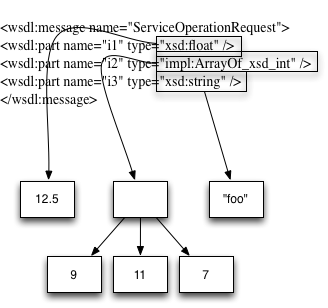
\includegraphics{./images/dipenta.png}
\caption{Genome representation \citep{Penta2007}. }
\label{fig:dipenta}
\end{figure}

\begin{figure}[h]
\centering
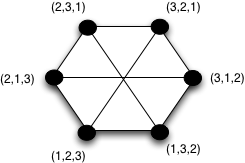
\includegraphics{./images/neighborhood.png}
\caption{ An example of neighborhood for a permutation \citep{Talbi2013}.}
\label{fig:sperneighborhood}
\end{figure}

\begin{figure}[h]
\begin{minipage}{.5\textwidth}
\centering
\includegraphics={./images/metaheuristc2.png}
\caption{Categories of metaheuristc combinations \citep{Puchinger2005} }
\label{fig:metaheuristc}
\end{minipage}
\begin{minipage}{.5\textwidth}
\centering
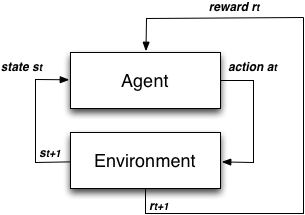
\includegraphics{./images/agentenv.png}
\caption{Example of an interaction between some agent and the environment}
\label{fig:agentenv}
\end{minipage}
\end{figure}

\begin{figure}
\begin{minipage}{.5\textwidth}
\centering
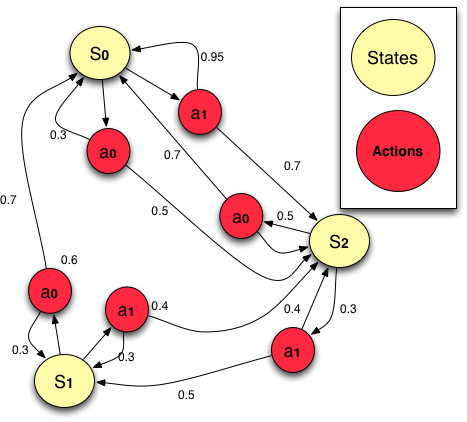
\includegraphics{./images/mdp1.png}
\caption{Example of a simple MDP with three states and two actions}
\label{fig:mdp}
\end{minipage}
\begin{minipage}{.5\textwidth}
\centering
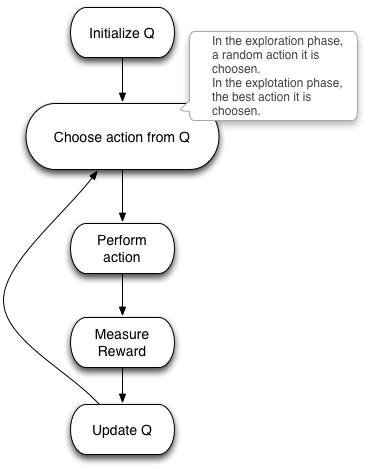
\includegraphics{./images/qalgo.png}
\caption{Q Learning algorithm}
\label{fig:qalgo}
\end{minipage}
\end{figure}


\begin{figure}[h]
\begin{minipage}{.5\textwidth}
\centering
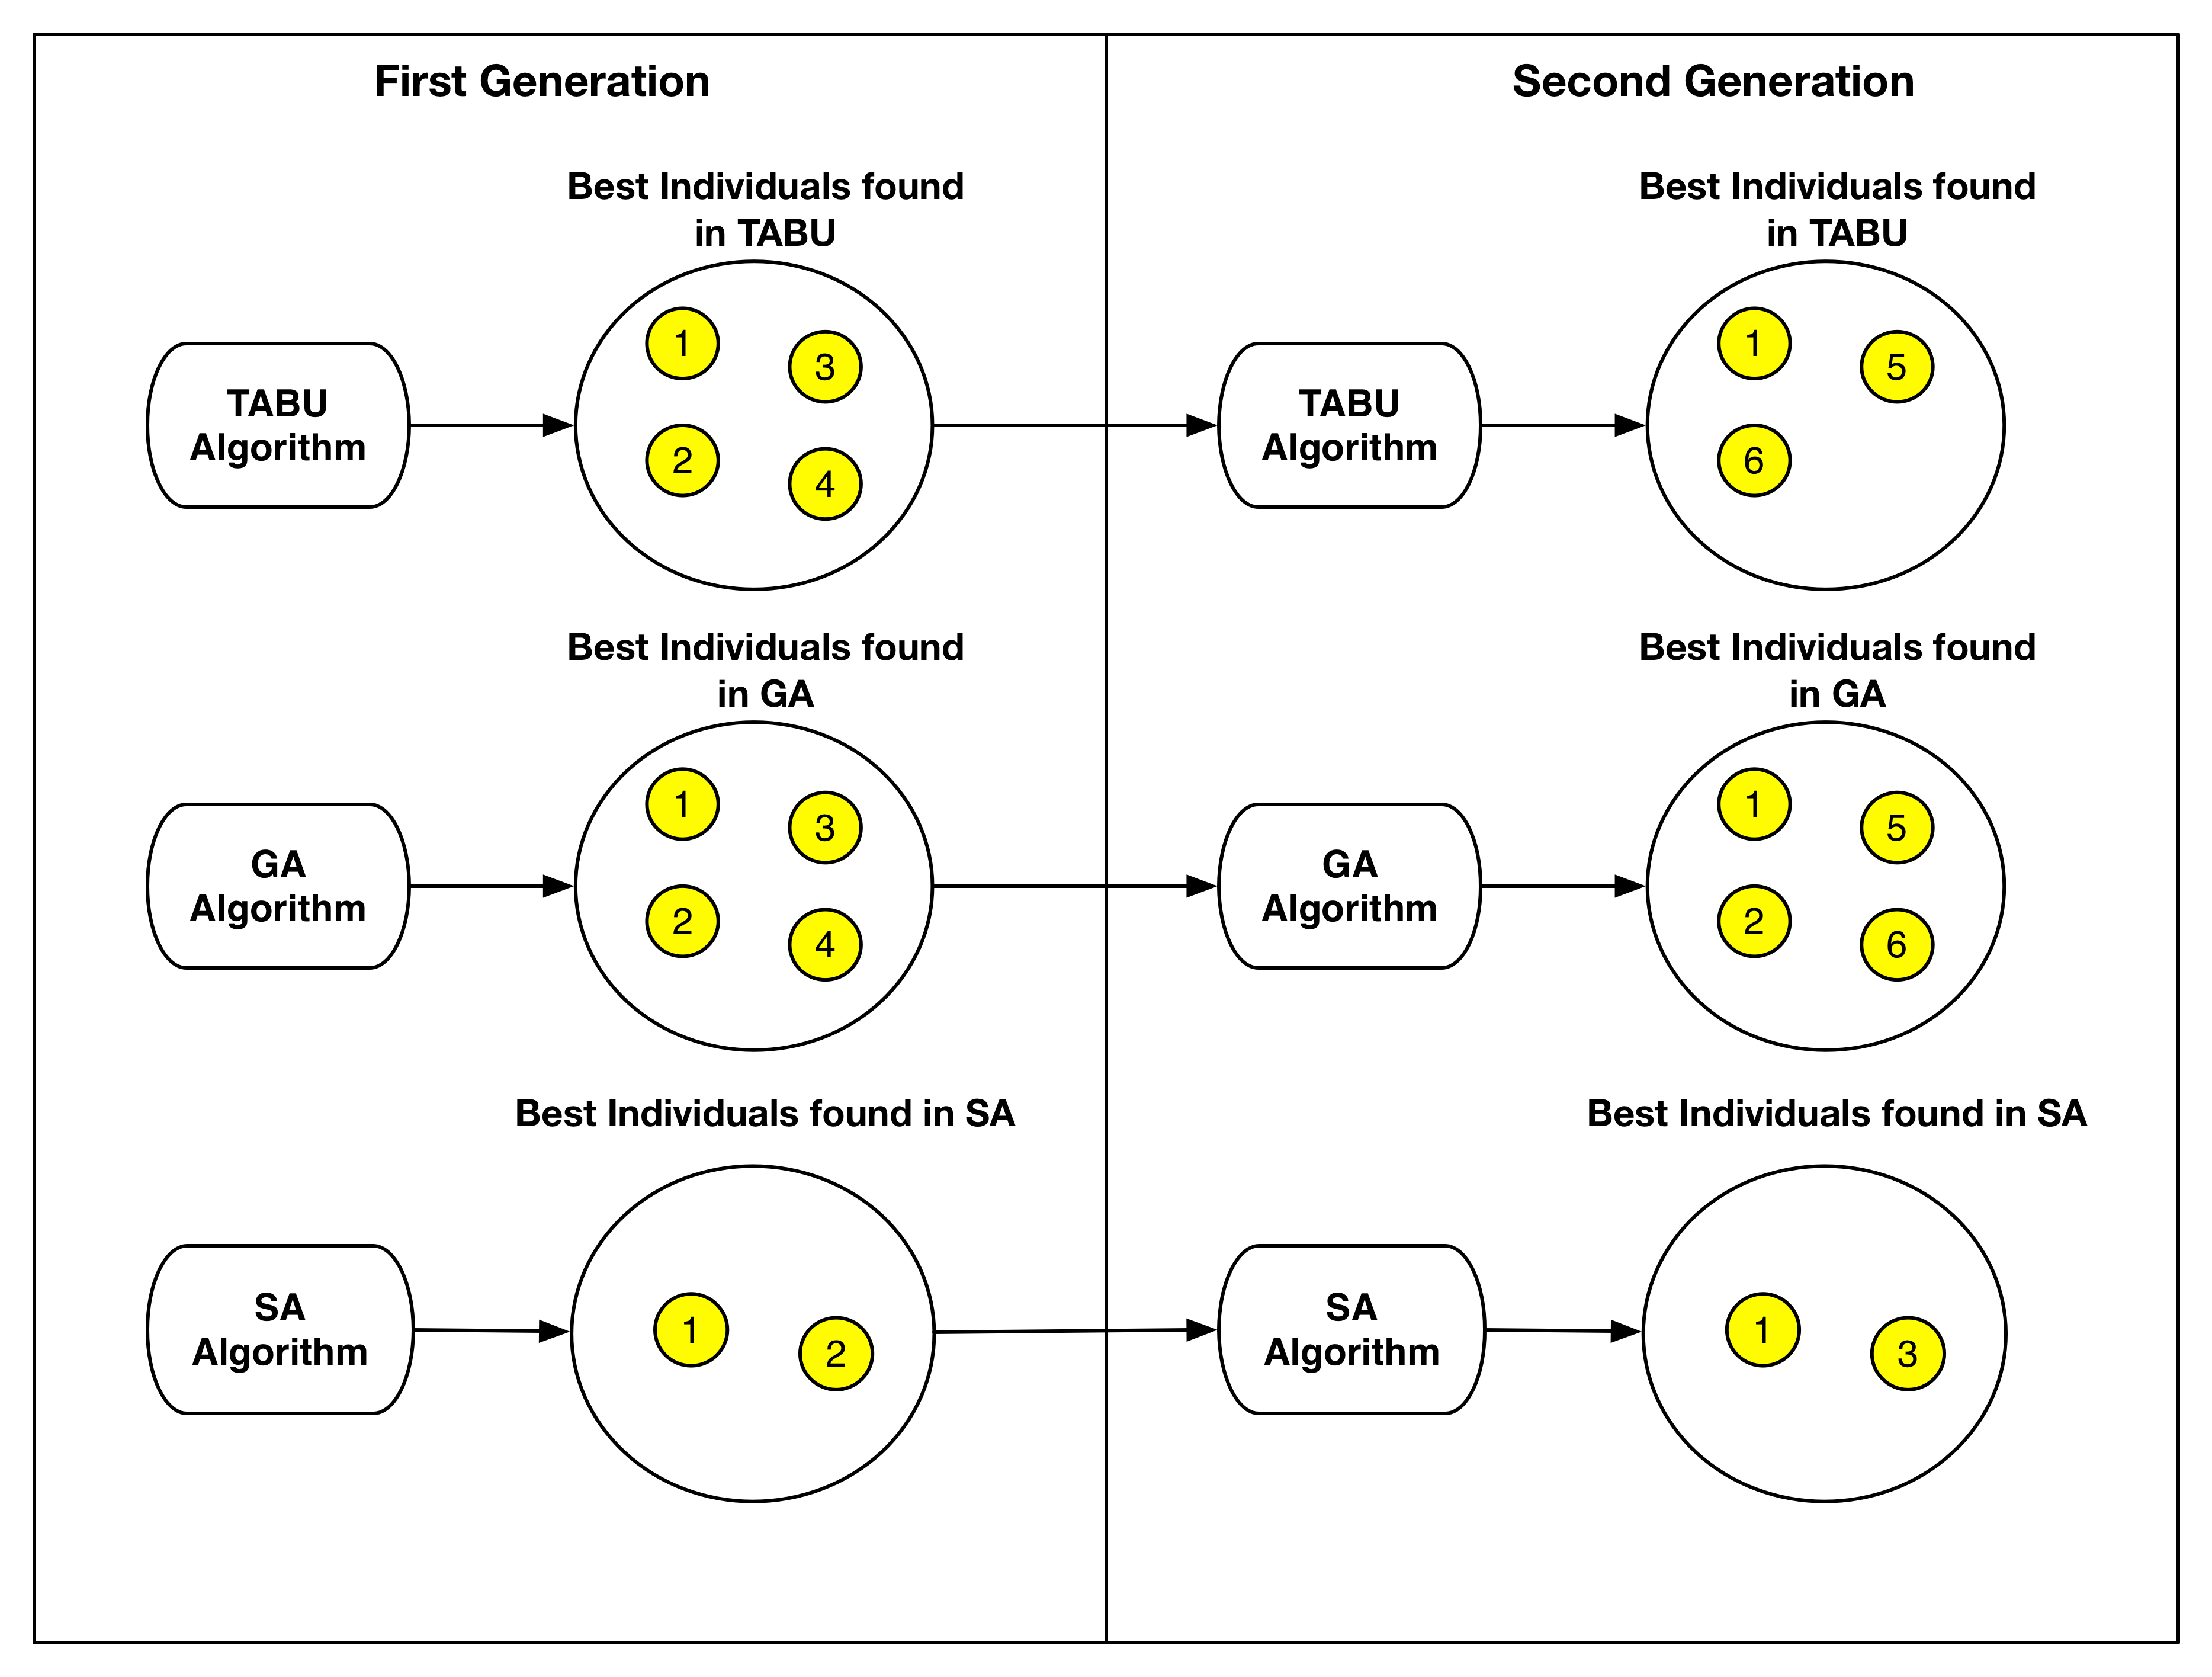
\includegraphics{./images/independ.png}
\caption{Use of the algorithms independently \citep{Gois2016}}
\label{fig:firstaproach}
\end{minipage}
\begin{minipage}{.5\textwidth}
\centering
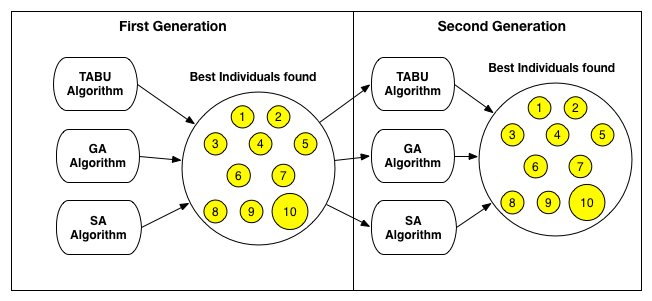
\includegraphics{./images/collaborative.png}
\caption{Use of the  algorithms collaboratively \citep{Gois2016}}
\label{fig:secondapproach}
\end{minipage}
\end{figure}

\begin{figure}[h]
\begin{minipage}{.5\textwidth}
\centering
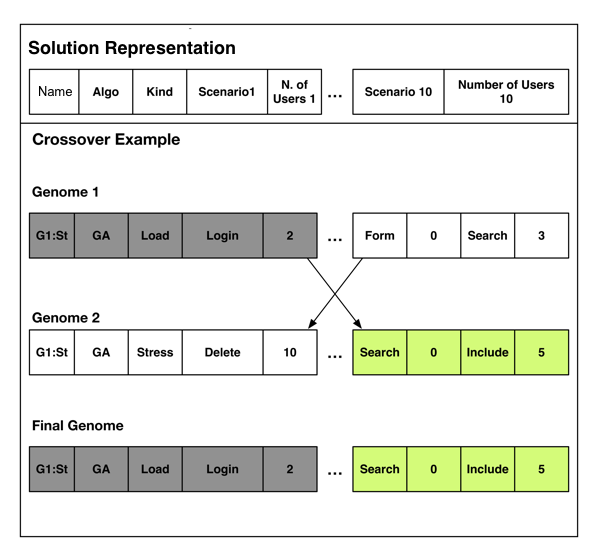
\includegraphics{./images/genomerepresentation1.png}
\caption{Solution representation and crossover example \citep{Gois2016}}
\label{fig:genomarepresentation}
\end{minipage}
\begin{minipage}{.5\textwidth}
\centering
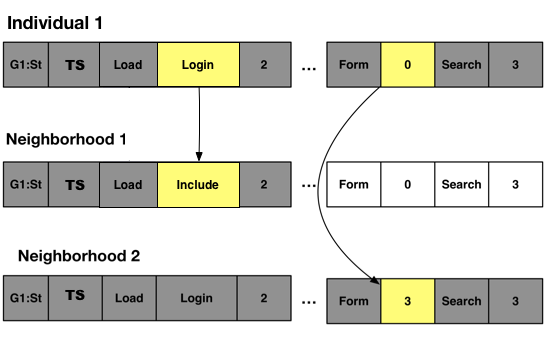
\includegraphics{./images/neighbor.png}
\caption{Tabu search and simulated annealing neighbor strategy \citep{Gois2016}}
\label{fig:neighbourtaby}
\end{minipage}
\end{figure}

\begin{figure}[h!]
\center
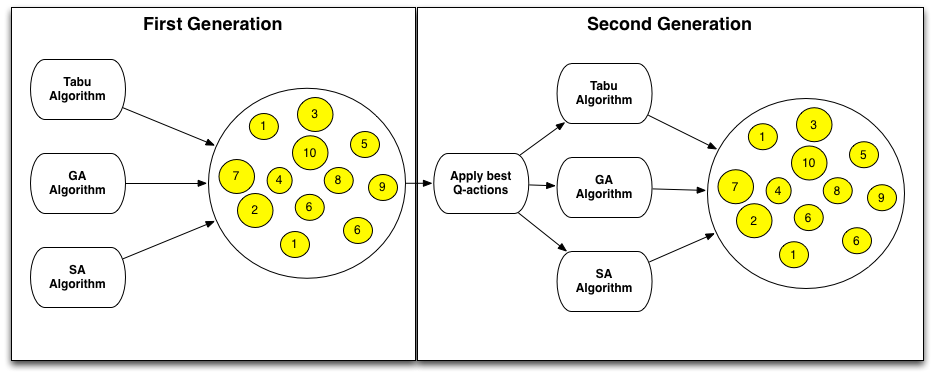
\includegraphics{./images/qhybrid.png}
\caption{Hybrid Metaheuristic with Q-Learning Approach}
\label{fig:hybridq}
\end{figure}

\begin{figure}[h!]
\begin{minipage}{.5\textwidth}
\center
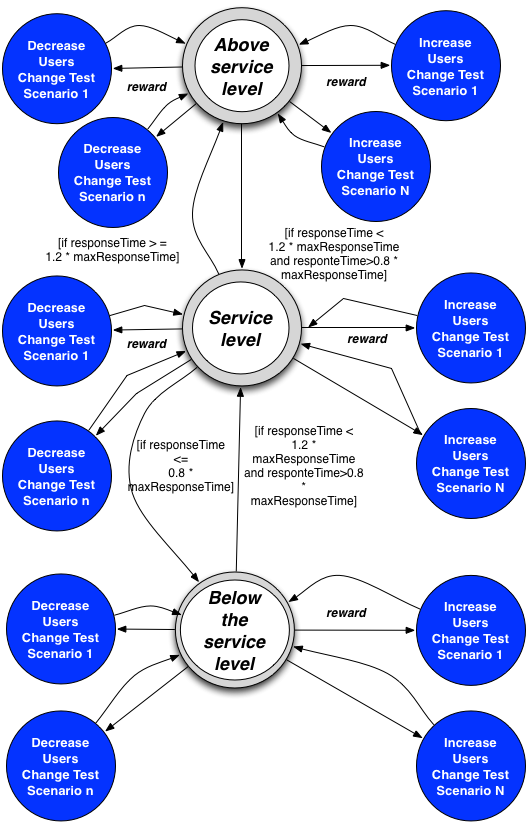
\includegraphics{./images/mdp3.png}
\caption{Markov Decision Process used by HybridQ}
\label{fig:mdphybridq}
\end{minipage}
\begin{minipage}{.5\textwidth}
\center
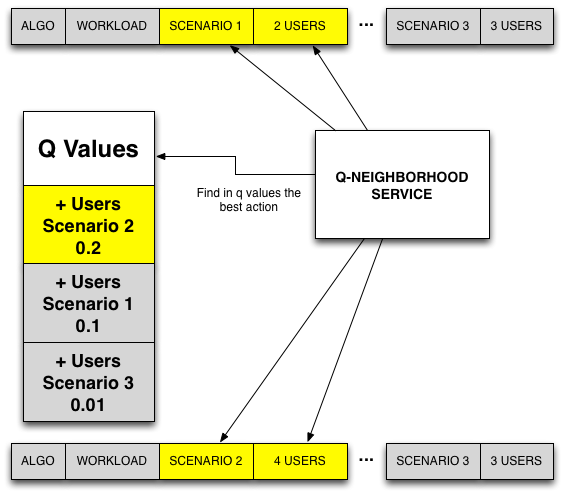
\includegraphics{./images/q-neighborservice.png}
\caption{HybridQ NeighborHood Service}
\label{fig:neighservice}
\end{minipage}
\end{figure}

\begin{figure}[h]
\begin{minipage}{.5\textwidth}
\center
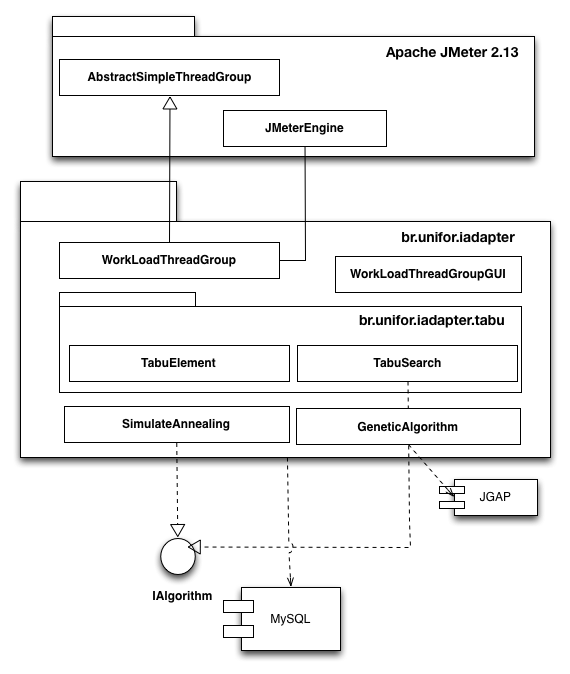
\includegraphics{./images/iadapter1.png}
\caption{IAdapter architecture}
\label{fig:iadapterarchitecture}
\end{minipage}
\begin{minipage}{.5\textwidth}
\centering
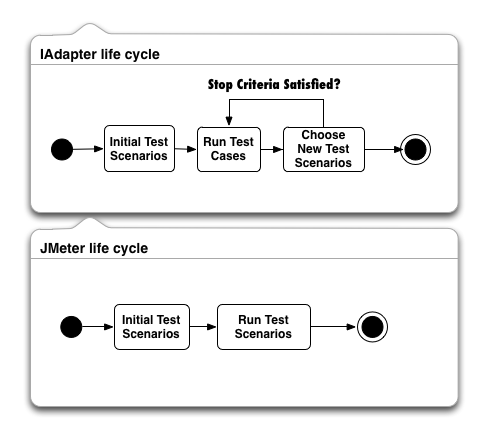
\includegraphics{./images/lifecycle2.png}
\caption{IAdapter life cycle}
\label{fig:iadapterlifecycle}
\end{minipage}
\end{figure}



\begin{figure}[h]
\centering
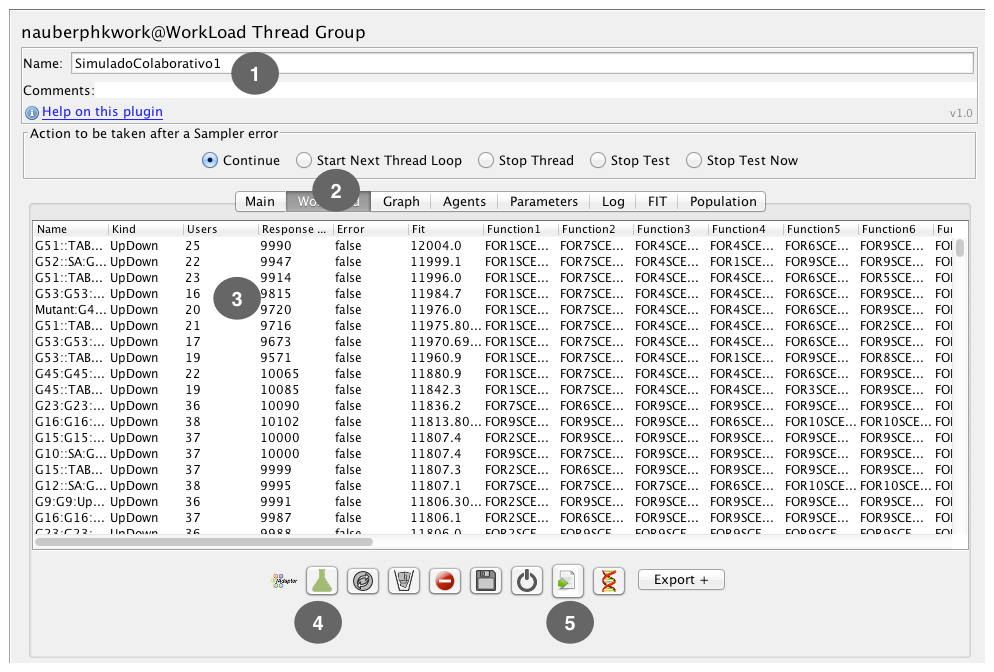
\includegraphics{./images/tela1iadapter.png}
\caption{WorkLoadThreadGroup component}
\label{fig:tela1iadapter}
\end{figure}

\begin{figure}[h]
\begin{minipage}{.5\textwidth}
\centering
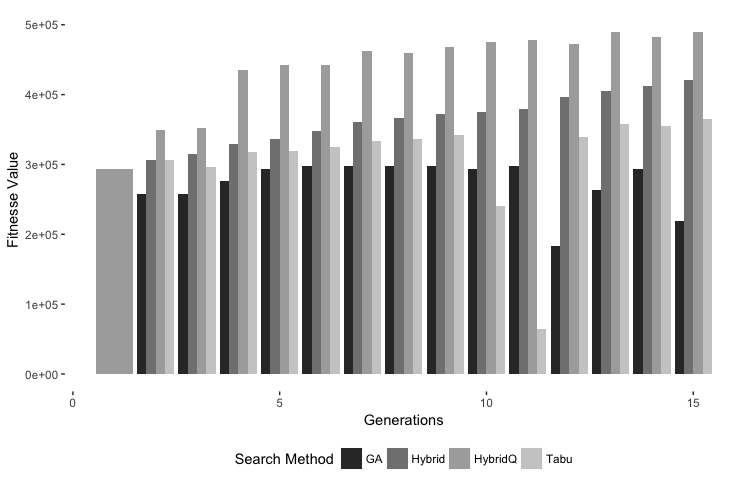
\includegraphics{./images/experiment1-1.png}
\caption{Fitness value obtained by Search Method }
\label{fig:fitnessbygeneration1}
\end{minipage}
\begin{minipage}{.5\textwidth}
\centering
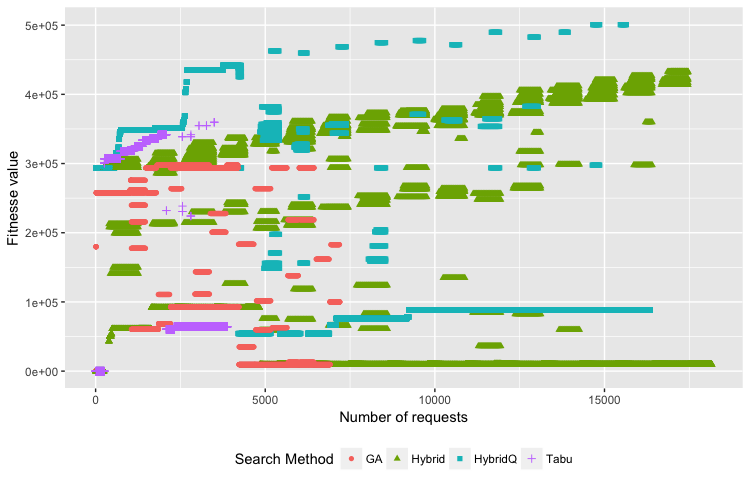
\includegraphics{./images/experiment1-3.png}
\caption{Number of requests by Search Method}
\label{fig:numberofrequestsbysearchmethod}
\end{minipage}
\end{figure}


\begin{figure}[h!]
\begin{minipage}{.5\textwidth}
\centering
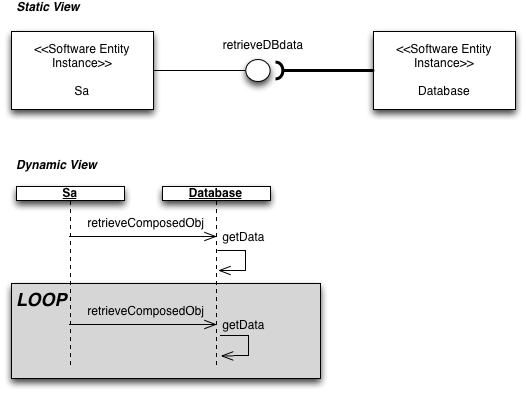
\includegraphics{./images/circuit.png}
\caption{Circuitous
Treasure Hunt sample \citep{Vetoio2011}}
\label{fig:circuit}
\end{minipage}
\begin{minipage}{.5\textwidth}
\centering
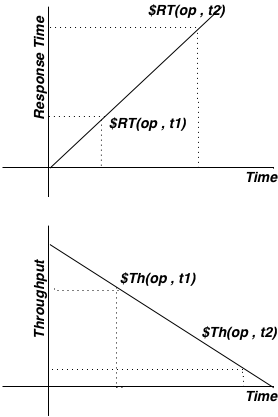
\includegraphics{./images/ramp.png}
\caption{The Ramp sample \citep{Vetoio2011}.}
\label{fig:ramp}
\end{minipage}
\end{figure}


\begin{figure}[h!]
\centering
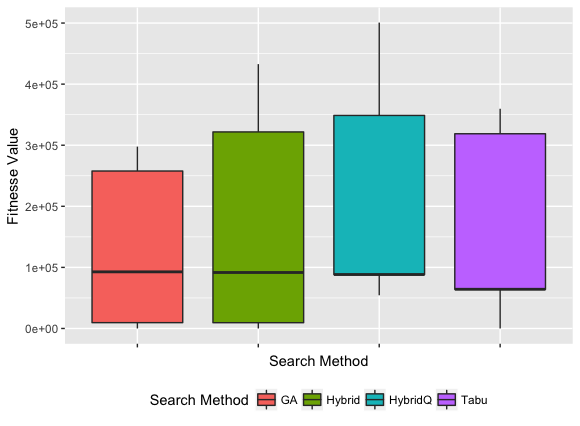
\includegraphics{./images/experiment1-4.png}
\caption{Average, median, maximum and minimal fitness value by Search Method}
\label{fig:boxplot1}
\end{figure}

\begin{figure}[h!]
\begin{minipage}{.5\textwidth}
\centering
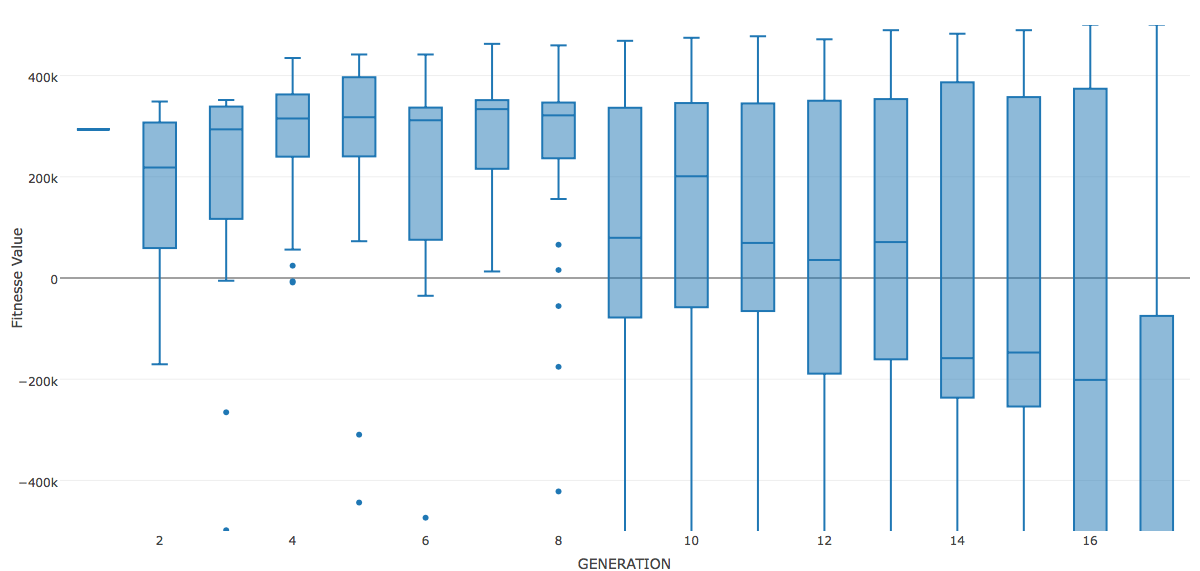
\includegraphics{./images/experiment1-5.png}
\caption{Fitness value by generation}
\label{fig:summaryboxplot1}
\end{minipage}
\begin{minipage}{.5\textwidth}
\centering
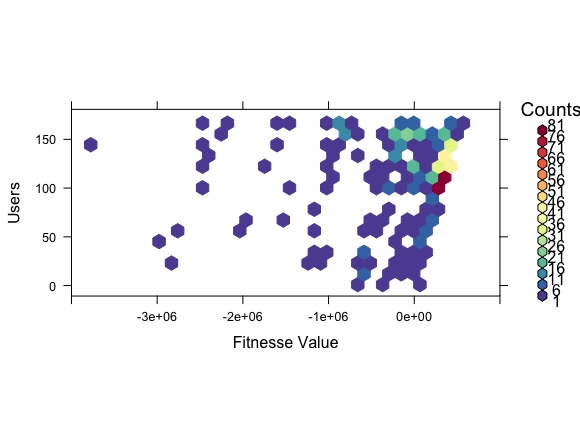
\includegraphics{./images/experiment1-6.png}
\caption{Density graph of number of users by fitness value}
\label{fig:density1}
\end{minipage}
\end{figure}

\begin{figure}[h!]
\centering
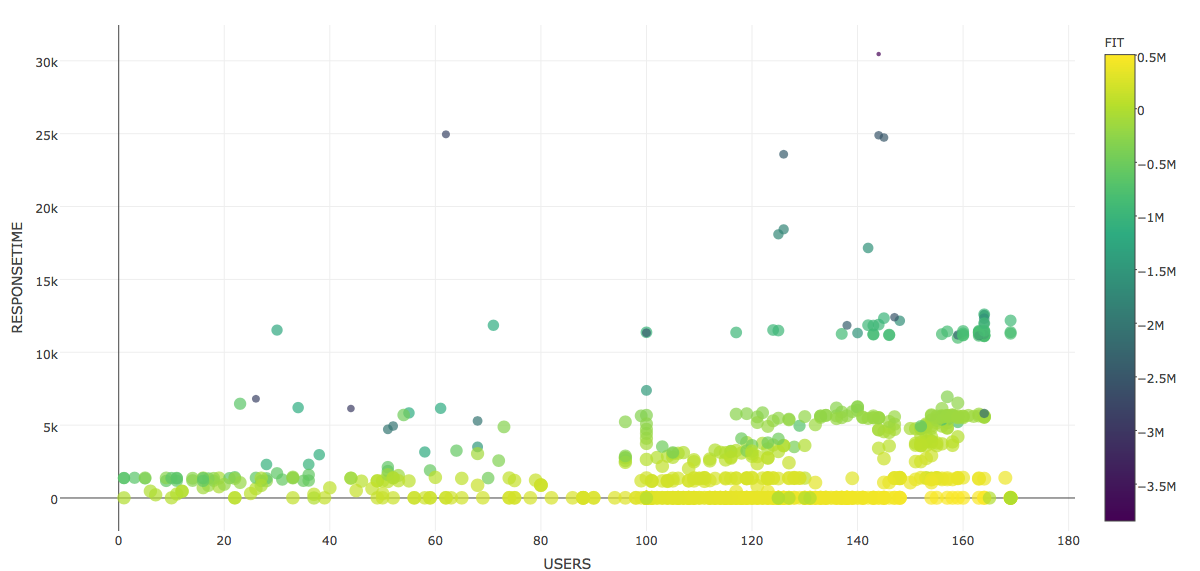
\includegraphics{./images/experiment1-7.png}
\caption{Response time by the number of users of individuals with Happy Scenario 1 and Happy Scenario 2}
\label{fig:responsetimegenerationalltests1}
\end{figure}
\begin{figure}[h]
\centering
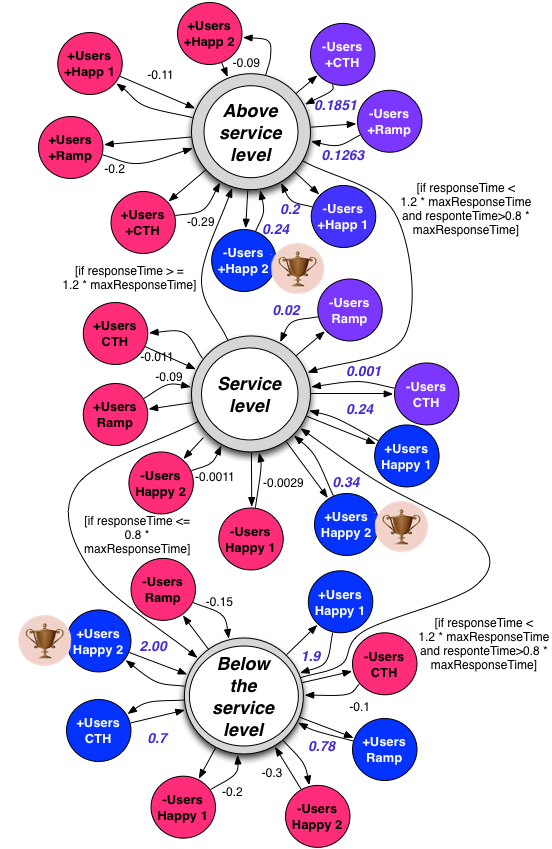
\includegraphics{./images/mdpexperiment.png}
\caption{Markov decision process of experiment with Circuitous Treasure and The Ramp antipatterns}
\label{fig:mdpexperiment1}
\end{figure}

\begin{figure}[h]
\begin{minipage}{.5\textwidth}
\centering
\includegraphics{./images/SearchSurface.png}
\caption{Response time of individuals found in the experiment by search method}
\label{fig:surface}
\end{minipage}
\begin{minipage}{.5\textwidth}
\centering
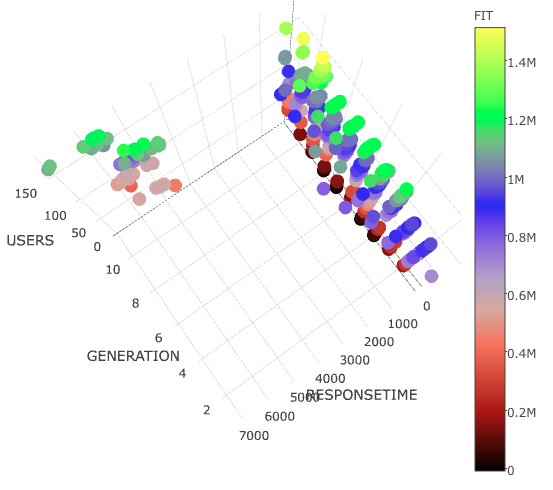
\includegraphics{./images/searchsurface2.png}
\caption{Response time of individuals found in the experiment by fitness value}
\label{fig:surface2}
\end{minipage}
\end{figure}

\begin{figure}[h]
\begin{minipage}{.5\textwidth}
\centering
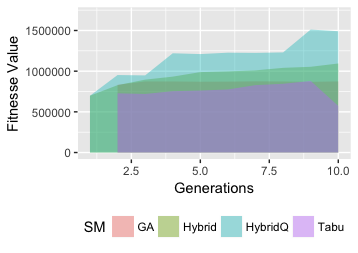
\includegraphics{./images/experiment3-1.png}
\caption{Fitness value by generation on JPetStore First experiment}
\label{fig:experiment31}
\end{minipage}
\begin{minipage}{.5\textwidth}
\centering
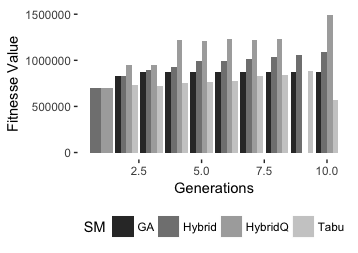
\includegraphics{./images/experiment3-2.png}
\caption{Fitness value by generation on JPetStore First experiment}
\label{fig:experiment32}
\end{minipage}
\end{figure}

\begin{figure}[h]
\begin{minipage}{.5\textwidth}
\centering
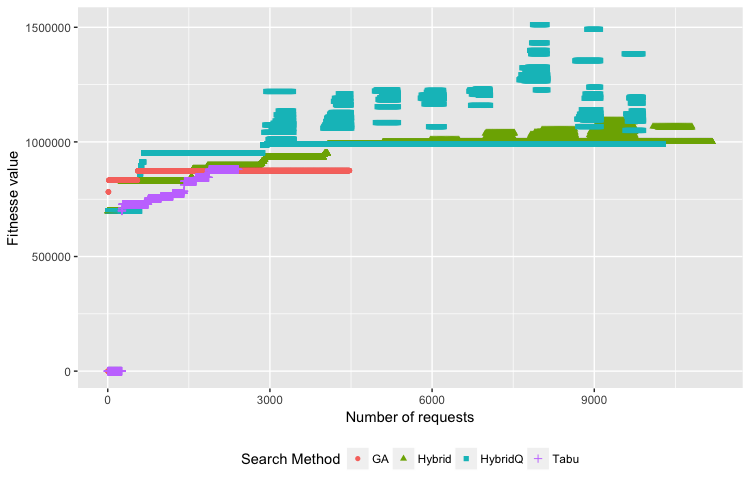
\includegraphics{./images/experiment3-3.png}
\caption{Number of requests by Search Method}
\label{fig:numberofrequestsbysearchmethod3}
\end{minipage}
\begin{minipage}{.5\textwidth}
\centering
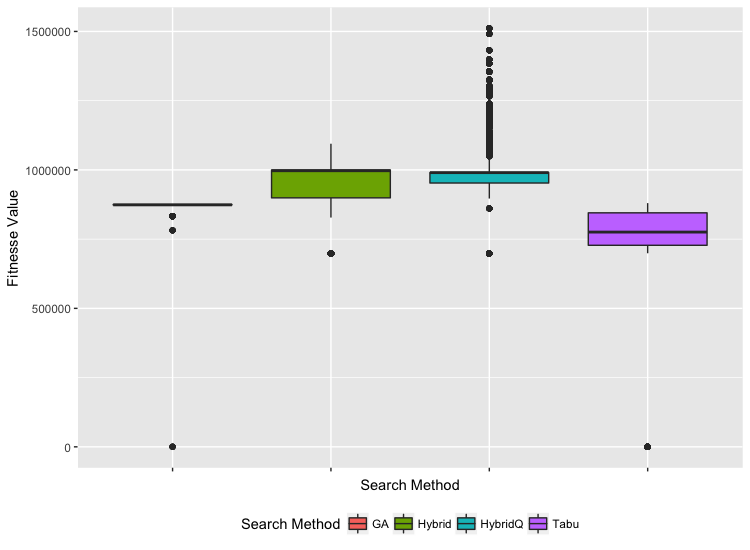
\includegraphics{./images/experiment3-4.png}
\caption{Fitness value by generation in all tests}
\label{fig:boxplot3}
\end{minipage}

\end{figure}

\end{backmatter}
\end{document}
